\documentclass[12pt, a4paper]{article}

% --- Paquetes ---
\usepackage[utf8]{inputenc}
\usepackage[spanish]{babel}
\usepackage[margin=2.5cm]{geometry}
\usepackage{amsmath, amssymb}
\usepackage{graphicx}
\usepackage{booktabs}
\usepackage{hyperref}
\usepackage{listings}
\usepackage{xcolor}
\usepackage{float}
\usepackage{pgfplots}
\pgfplotsset{compat=1.18}

% --- Configuración de Colores para Código ---
\definecolor{codegreen}{rgb}{0,0.6,0}
\definecolor{codegray}{rgb}{0.5,0.5,0.5}
\definecolor{codepurple}{rgb}{0.58,0,0.82}
\lstset{
    commentstyle=\color{codegreen},
    keywordstyle=\color{magenta},
    numberstyle=\tiny\color{codegray},
    stringstyle=\color{codepurple},
    basicstyle=\ttfamily\small,
    breaklines=true,
    captionpos=b,
    numbers=left,
    showstringspaces=false
}

% --- Título ---
\title{Tarea 1: Algoritmos de Ordenamiento Secuenciales y Paralelos}
\author{Javier Torres \& Juan Umaña \& Benjamin Jimenez \\ \small Sistemas Distribuidos y Paralelos \\ \small Universidad de Concepción}
\date{Abril 2026}

\begin{document}

\maketitle

\begin{abstract}
Este informe presenta la implementación, análisis y comparación de algoritmos de ordenamiento Mergesort y K-way Mergesort en sus variantes secuenciales y paralelas. Se utiliza el estándar OpenMP para la paralelización y se emplea la técnica de Merge por Ranks para optimizar la fusión de subarreglos. Los resultados experimentales, obtenidos sobre un procesador AMD Ryzen 5 8600G, validan el análisis teórico de Work y Span, demostrando una escalabilidad significativa en escenarios con alta carga de datos.
\end{abstract}

\section{Introducción}
El problema del ordenamiento es fundamental en la computación paralela, sirviendo como caso de estudio para el balance de carga, la granularidad y la gestión de memoria. En este trabajo, se exploran estrategias para minimizar el \textit{Span} de los algoritmos clásicos, pasando de una recursión paralela simple a una implementación completa que paraleliza incluso la operación de mezcla (\textit{merge}).

\section{Descripción de Algoritmos}

\subsection{Mergesort Secuencial y Paralelo}
El Mergesort se basa en el paradigma de divide-and-conquer. La versión paralela implementada utiliza tareas (\textit{tasks}) de OpenMP para procesar las llamadas recursivas de forma concurrente. Se introduce un parámetro de \textbf{granularidad} para evitar el sobrecosto de creación de hilos en subproblemas pequeños.

\subsection{Merge Paralelo por Ranks}
Para superar el cuello de botella del merge secuencial de $O(n)$, se implementó el algoritmo de \textbf{Merge Path}. Este utiliza búsqueda binaria para calcular los \textit{ranks} (puntos de corte) en los subarreglos ordenados, permitiendo que múltiples hilos fusionen tramos independientes de forma simultánea.

\subsection{K-way Mergesort}
A diferencia del Mergesort binario, el K-way divide el arreglo en $k$ bloques. La versión paralela completa combina la división en $k$ partes con el merge paralelo interno, maximizando el aprovechamiento de los núcleos disponibles.

\section{Análisis Teórico}

\subsection{Modelo PRAM y Work/Span}
Considerando un arreglo de tamaño $n$ y $p$ procesadores:
\begin{itemize}
    \item \textbf{Mergesort Paralelo (Merge Secuencial):}
    \begin{itemize}
        \item $W(n) = O(n \log n)$
        \item $S(n) = S(n/2) + O(n) = O(n)$
    \end{itemize}
    \item \textbf{Merge Paralelo por Ranks:}
    \begin{itemize}
        \item $W_{merge}(n) = O(n)$
        \item $S_{merge}(n) = O(\log n)$
    \end{itemize}
    \item \textbf{Versión Paralela Completa:}
    \begin{itemize}
        \item $S(n) = S(n/k) + O(\log n) = O(\log^2 n)$ (para $k$ constante).
    \end{itemize}
\end{itemize}

\subsection{Teorema de Brent}
Según el Teorema de Brent, el tiempo de ejecución estimado es $T_p \leq \frac{W(n)}{p} + S(n)$. En nuestra implementación completa, esto se traduce en $T_p \approx \frac{n \log n}{p} + \log^2 n$, lo que predice una alta eficiencia para valores grandes de $n$.

\section{Metodología Experimental}

\subsection{Entorno de Ejecución}
Las pruebas se realizaron en un procesador **AMD Ryzen 5 8600G** (6 núcleos físicos, 12 hilos) con 32 GB de RAM DDR5. Se utilizó el compilador `g++` con el flag de optimización `-O3`.

\subsection{Parámetros de Prueba}
\begin{itemize}
    \item Tamaños de arreglo: $n \in \{2^{20}, 2^{22}, 2^{24}, 2^{26}\}$.
    \item Hilos: $p \in \{1, 2, 4, 8\}$.
    \item Granularidad: 8192 elementos.
\end{itemize}

\clearpage

\section{Resultados y Discusión}

\begin{figure}[H]
    \centering
    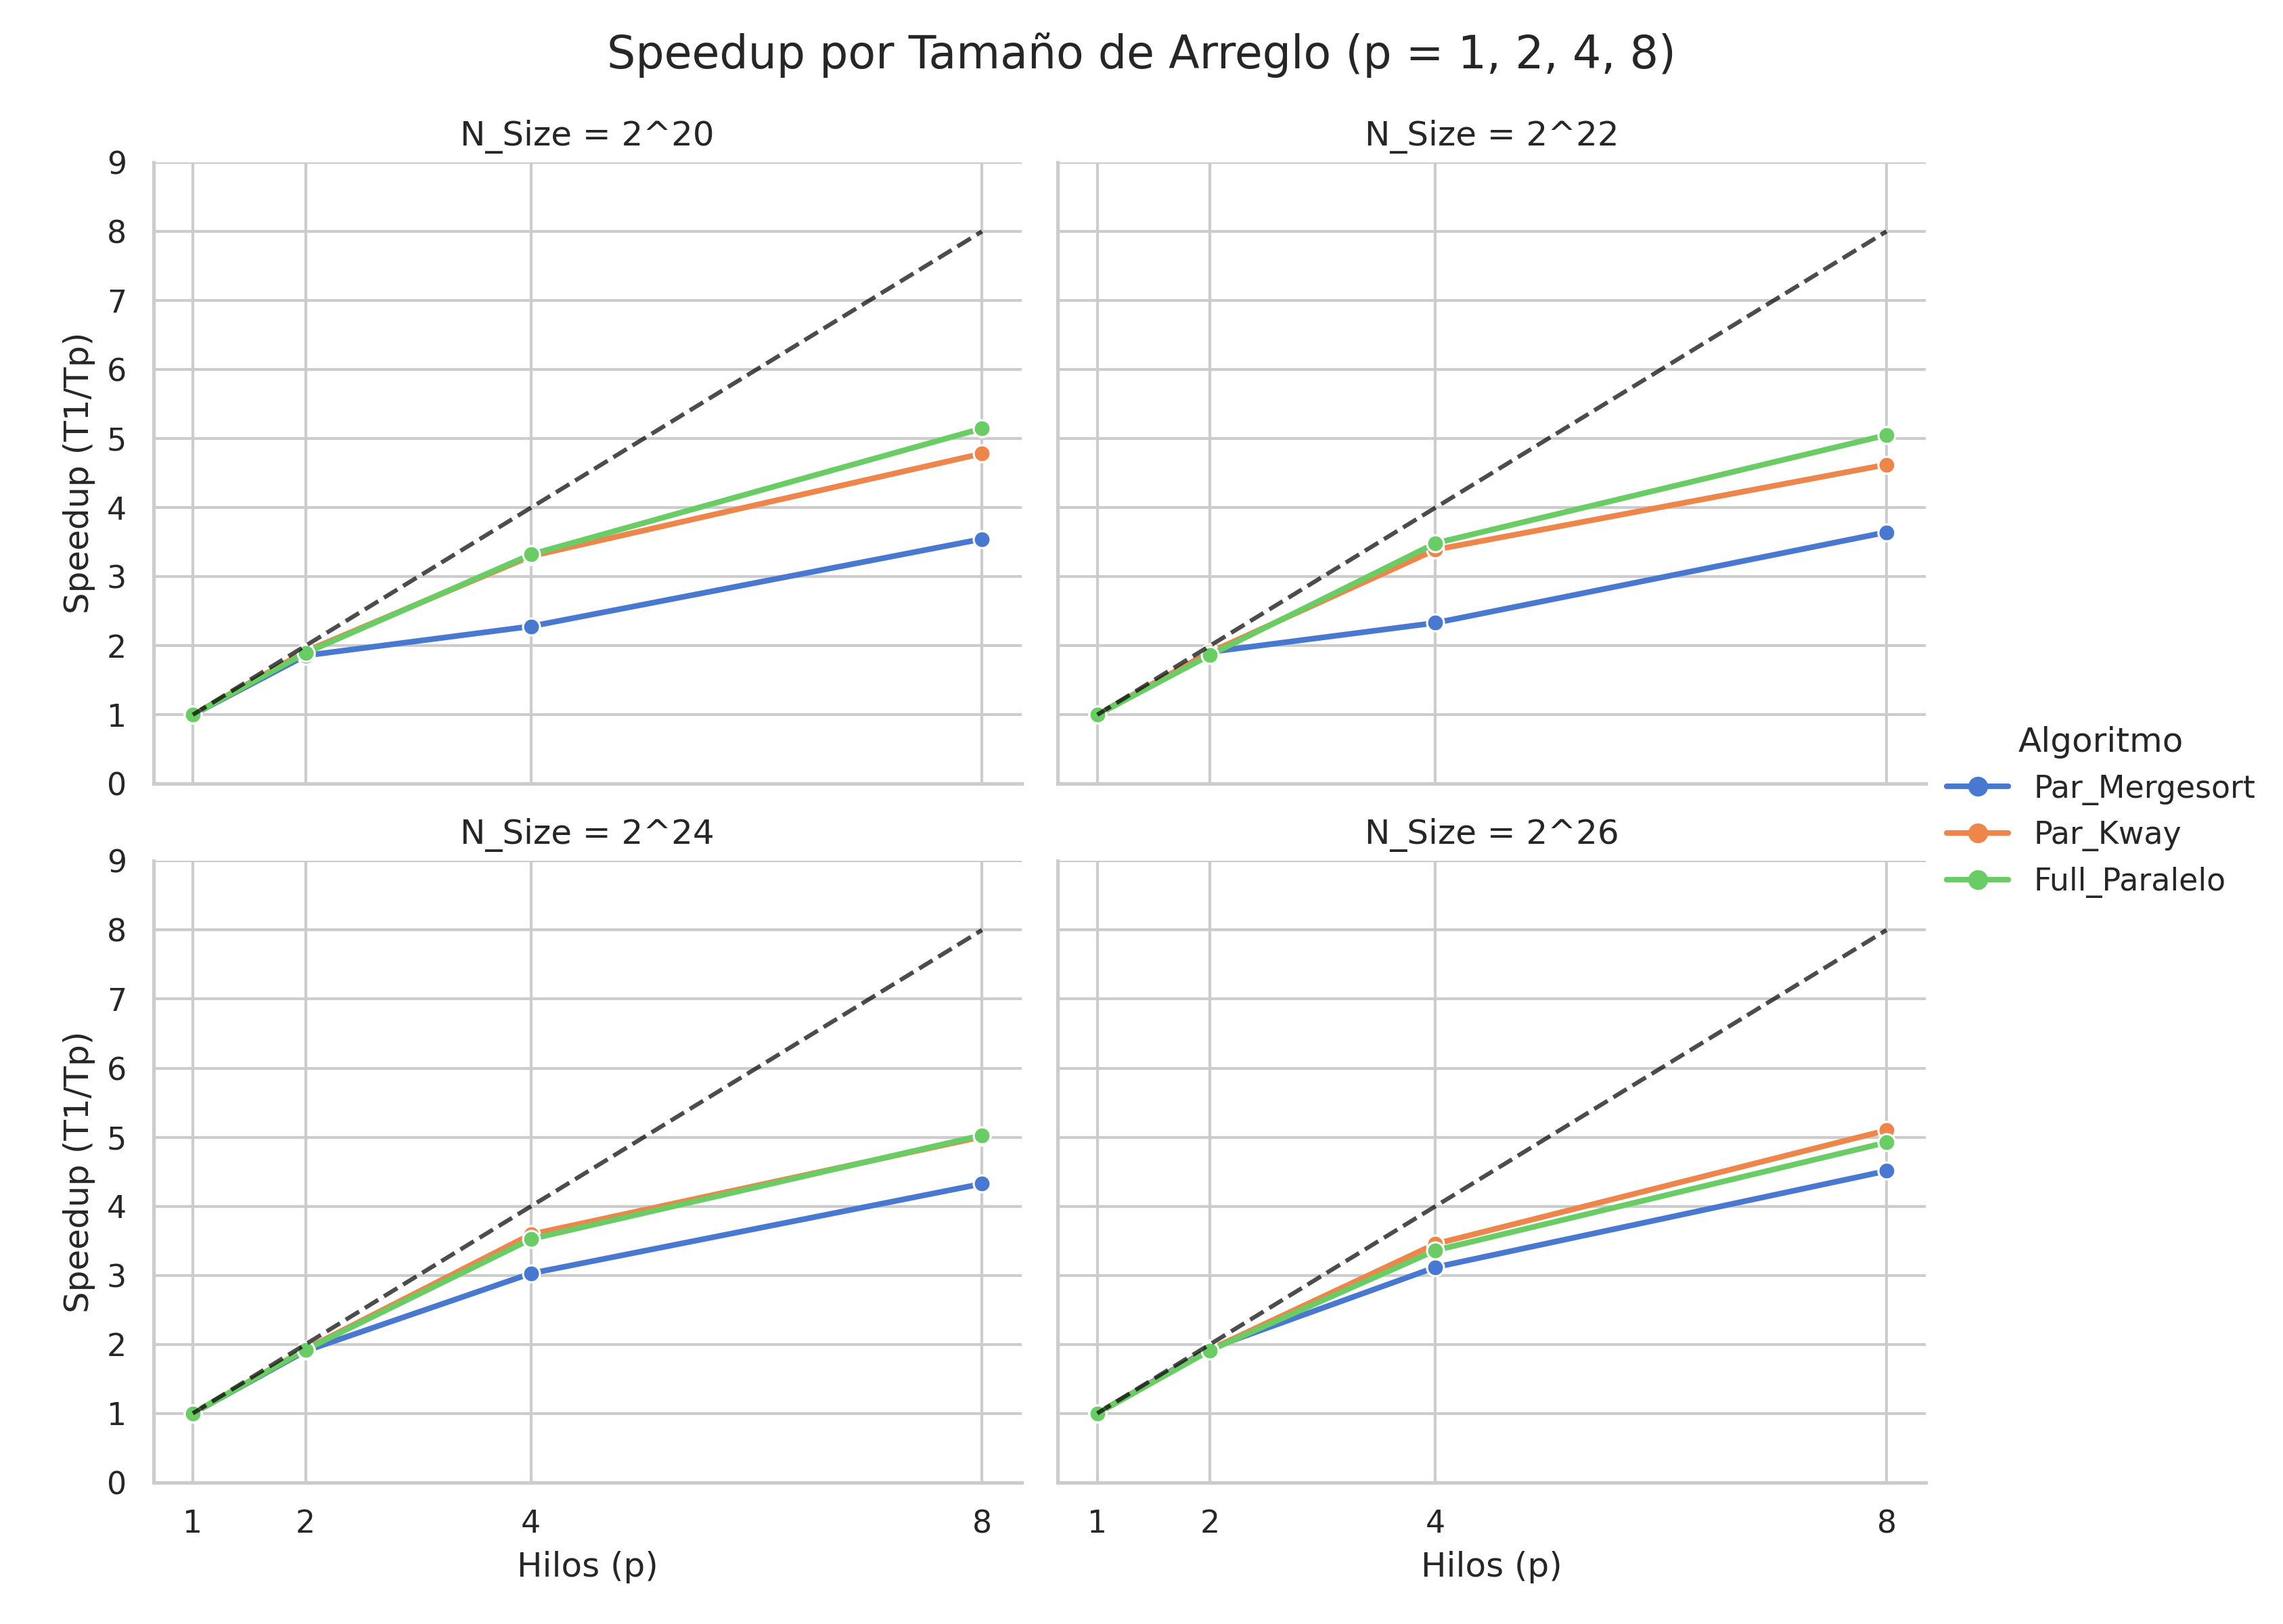
\includegraphics[width=1.0\textwidth]{grafico_speedup_facet.png}
    \caption{Speedup obtenido para diferentes tamaños de arreglo y número de hilos.}
\end{figure}

\begin{figure}[H]
    \centering
    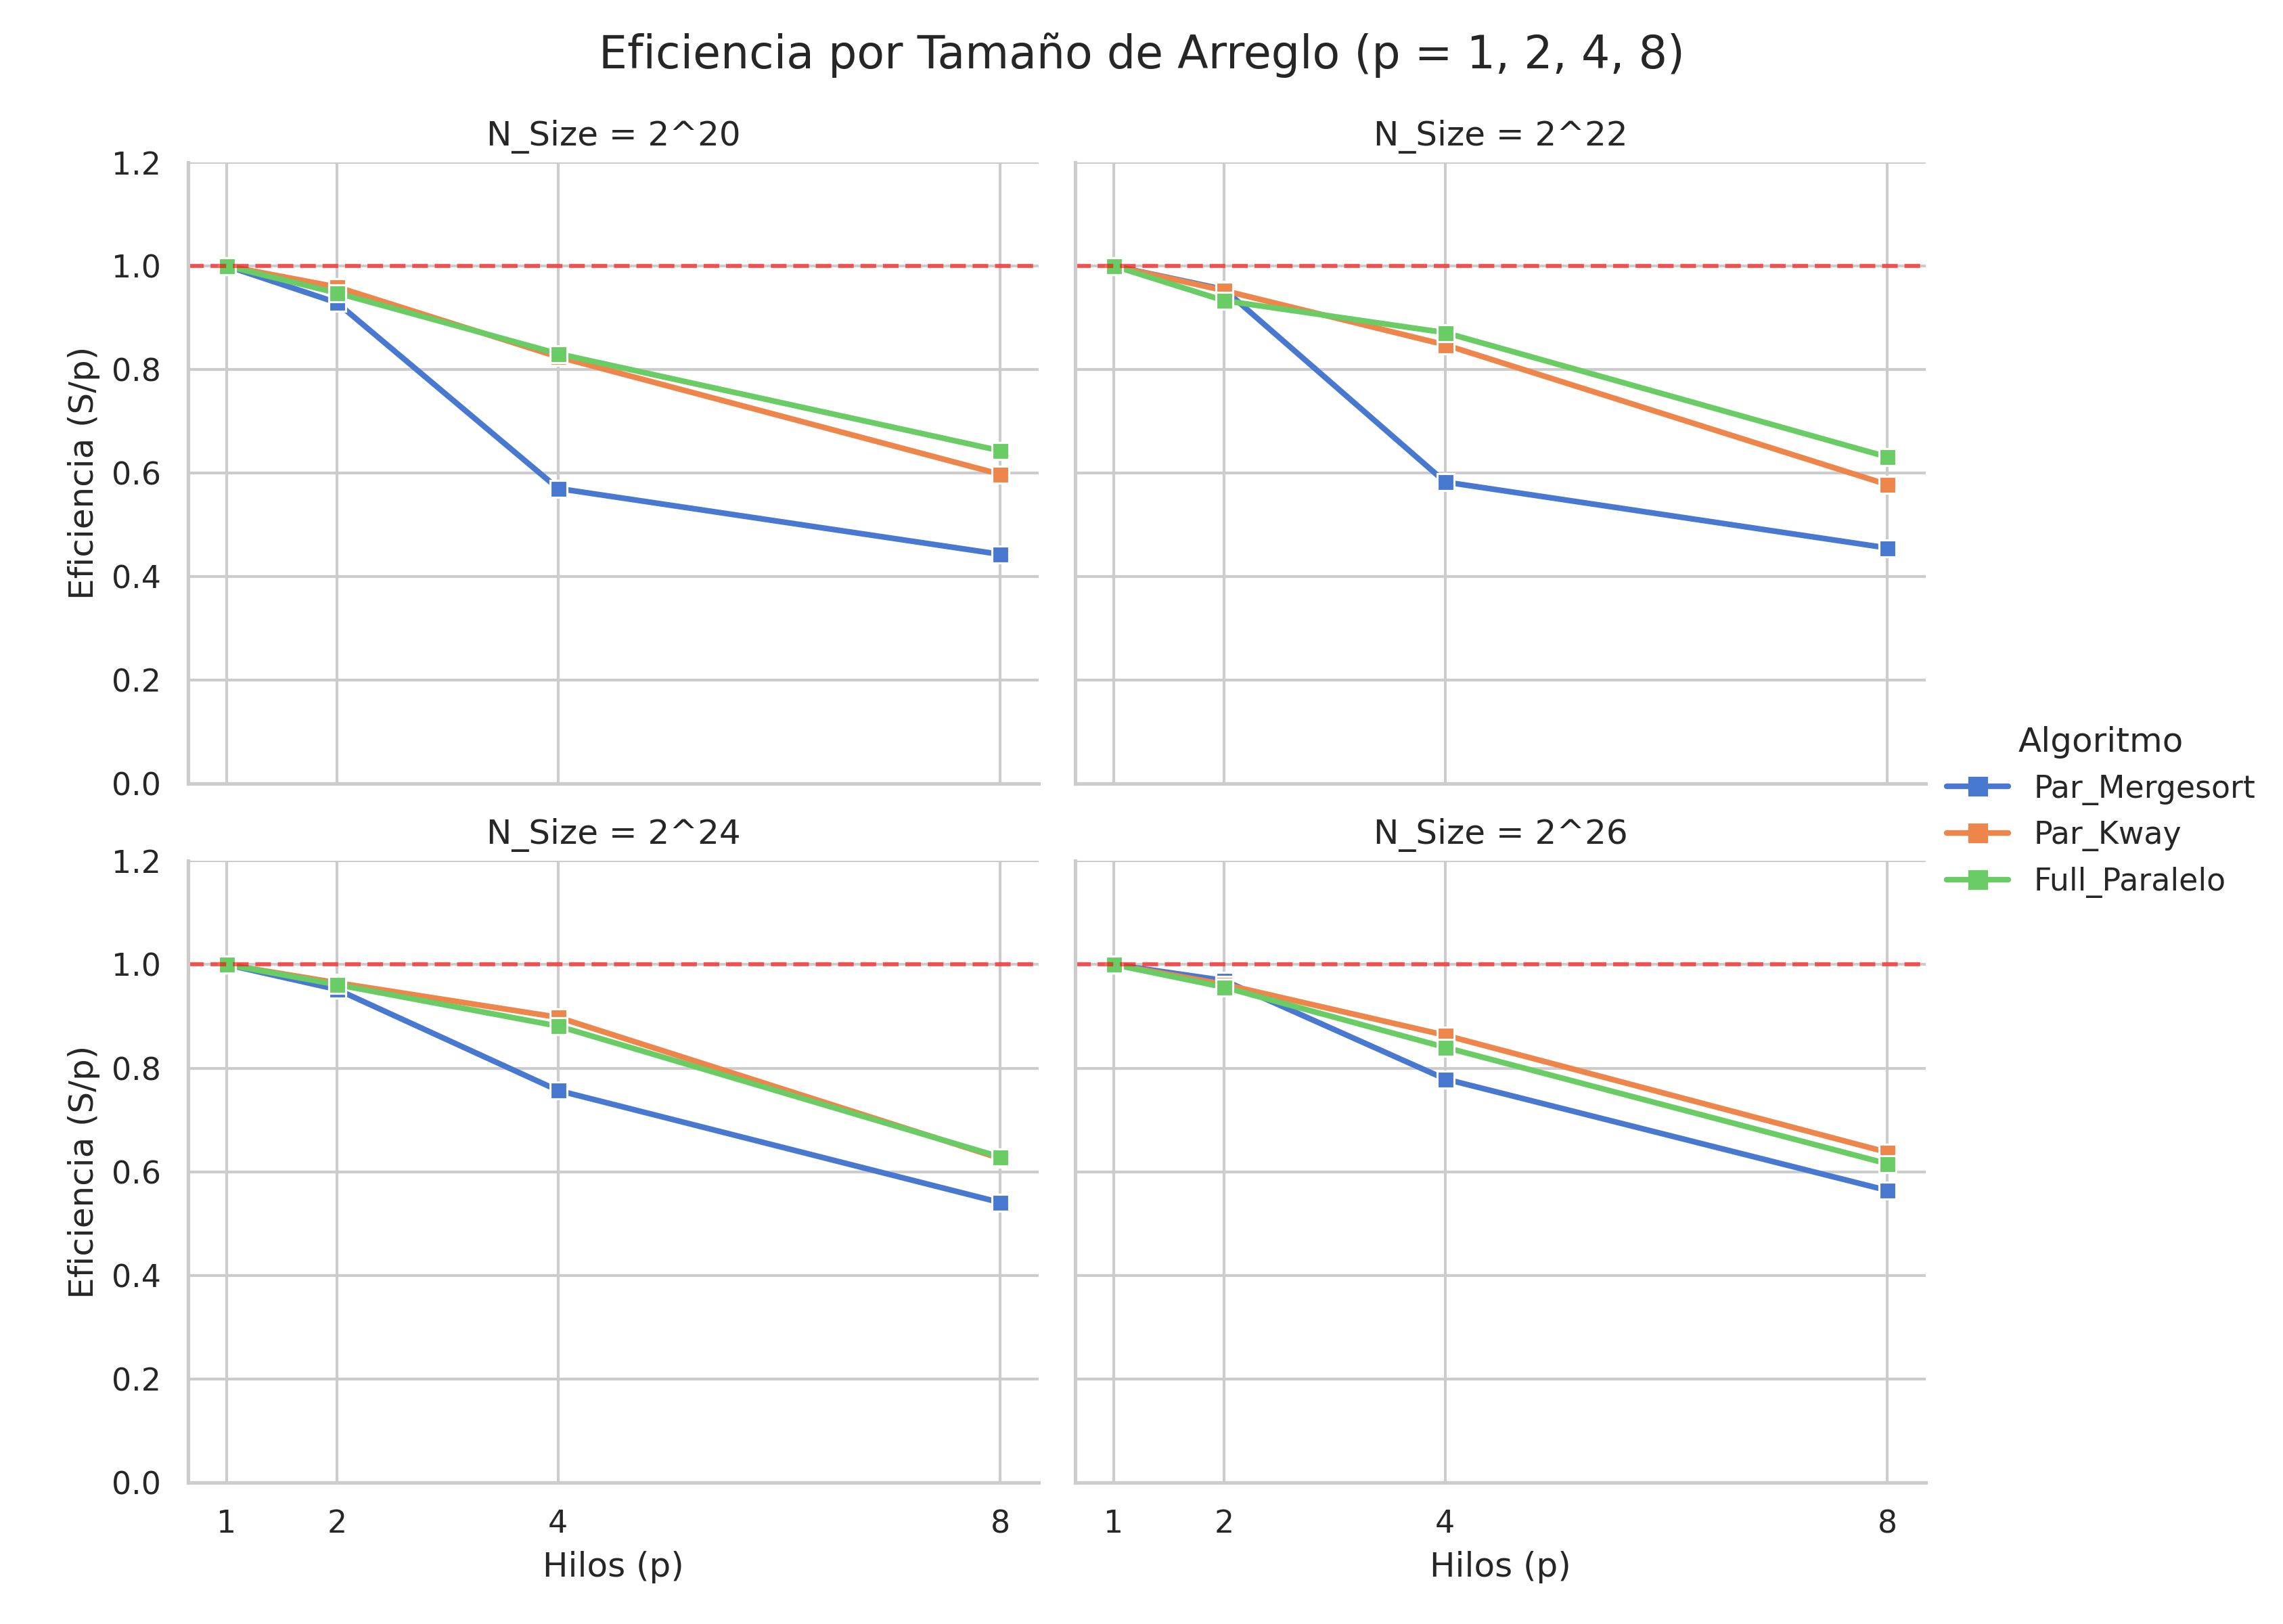
\includegraphics[width=1.0\textwidth]{grafico_eficiencia_facet.png}
    \caption{Eficiencia relativa en función del número de hilos y tamaño del arreglo.}
\end{figure}


% Ejemplo de inclusión de tabla (puedes completar con tus datos reales)
\begin{figure}[hbt!]
    \centering
    \begin{tikzpicture}
        \begin{axis}[
            title={Speedup para $N = 2^{26}$},
            xlabel={Número de Hilos ($p$)},
            ylabel={Speedup ($T_1 / T_p$)},
            xmin=1, xmax=8,
            ymin=1, ymax=8,
            xtick={1, 2, 4, 8},
            ytick={1, 2, 3, 4, 5, 6, 7, 8},
            legend pos=north west,
            grid=both,
            grid style={line width=.1pt, draw=gray!10},
            major grid style={line width=.2pt,draw=gray!50},
            width=10cm,
            height=7cm
        ]
        
        % Ideal teórica
        \addplot[color=black, dashed, thick, domain=1:8] {x};
        \addlegendentry{Ideal ($S_p = p$)}
        
        % Par_Mergesort
        \addplot[color=blue, mark=square*, thick] coordinates {
            (1,1.0000) (2,1.9383) (4,3.1162) (8,4.5110)
        };
        \addlegendentry{Par\_Mergesort}
        
        % Par_Kway
        \addplot[color=orange, mark=triangle*, thick] coordinates {
            (1,1.0000) (2,1.9236) (4,3.4543) (8,5.0996)
        };
        \addlegendentry{Par\_Kway}
        
        % Full_Paralelo
        \addplot[color=green!60!black, mark=*, thick] coordinates {
            (1,1.0000) (2,1.9124) (4,3.3606) (8,4.9240)
        };
        \addlegendentry{Full\_Paralelo}
        
        \end{axis}
    \end{tikzpicture}
    \caption{Escalabilidad de los algoritmos para el tamaño máximo de arreglo analizado. Se observa un estancamiento de la eficiencia al utilizar 8 hilos, alejándose de la curva ideal.}
    \label{fig:speedup_n26}
\end{figure}

\section{Conclusiones}
La implementación del merge paralelo es fundamental para lograr una escalabilidad real en arquitecturas multinúcleo. Los resultados demuestran que, aunque el \textit{Work} se mantiene constante, la drástica reducción del \textit{Span} permite que el sistema se acerque al speedup ideal en problemas de gran tamaño.

\end{document}
